\section{INTRODUCTION}
\label{sec:intro}

\begin{figure*}[h!]
    \centering
    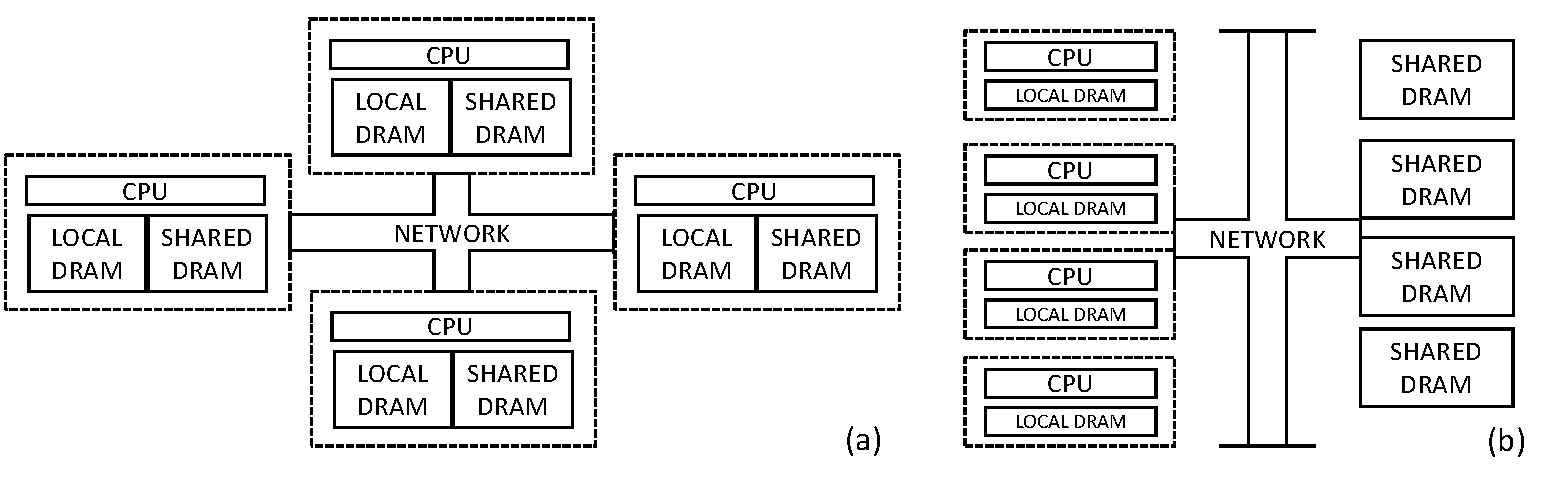
\includegraphics[width=.9\linewidth]{fig/architecture.pdf}
    \caption{(too big?) Shows (a) software-disaggregated 
    architecture where disaggregated memory is pooled from 
    traditional servers as opposed to the (b) hardware-disaggregated
    design where most memory is decoupled in hardware.}
    \label{fig:architecture}
\end{figure*}

With the tremendous growth of computing in the past two 
decades, applications have become both data-intensive 
and latency-sensitive, which gave rise to in-memory 
computing in lieu of going to the disk. 
This led to memory-intensive 
applications whose memory needs on a server outweigh the 
processor needs, introducing a skew in resource usage.
However, traditional servers come with fixed processor 
and memory resources that does not allow dynamically
resizing memory. This was generally solved by swapping 
to disk but disk speeds were really slow compared to memory 
affecting performance. 
At the same time, the diversification of computing usecases 
introduced a high heterogeneity of applications (e.g., cloud 
computing) with varying memory needs in proportion to 
the CPU, leaving some of the traditional servers in a data center  
with underutilized memory and others with not enough; the result
being inefficient memory utilization in the cluster and hence,
increased cost of ownership. Decoupling memory would allow 
applications to be more elastic in their memory usage and 
improve the memory utilization of the cluster at the same time.
Memory disaggregation involves such (logical or physical) 
decoupling of memory resources in a cluster from other 
(processor) resources. 
% \anil{there are other benefits to memory disaggregation...}

One way to alleviate memory pressure is to scale out and 
build a distributed application that runs on multiple nodes and 
adjust itself to the memory restrictions on the individual 
nodes. Indeed, there are many platforms that provide distributed 
memory management for such applications like distributed key-value 
stores~\cite{Ousterhout2010,Lim2012,Novakovic2016,Kalia2015},
distributed shared memory (DSM) 
systems~\cite{treadmarks,dsm1,farm,gam}, etc. These systems 
provide a globally accessible interface for all servers where  
the focus is on providing fine-grained memory sharing and 
a reasonable consistency model for distributed applications. 
An alternative is to extend the private memory space 
of (single-node) applications a la 
remote swapping systems~\cite{gms,cashmere} that transparently
swap application pages to remote memory without any notion 
of sharing across servers (i.e., their memory 
consistency model stops with cache coherence protocols on a 
single server). In this report, we focus 
on the latter kind where the stress is more on perfomant 
remote access mechanisms and efficient memory management for 
individual applications and less on memory sharing and 
consistency across servers.

As the networks become faster and technologies such as 
RDMA~\cite{farm,rocev2} arrive to commodity clusters, 
the remote access latencies are inching closer to native 
DRAM latencies (which, on the contrary, are nearing 
saturation~\cite{Aguilera2017}), making remote memory more 
accessible for applications, performance-wise~\cite{netdisagg}. 
Consequently, there has been a renewed interest in 
recent years in building remote memory 
systems~\cite{infiniswap,zswap,leap,fastswap,
legoos,kona,aifm,semeru,remregions,literdma}.
Traditional way of memory disaggregation is to pool/track  
unused memory across the cluster in software 
and use it to complement memory on the memory-hungry servers.
This is still popular with work on remote swapping systems 
continuing to this day~\cite{infiniswap,fastswap,zswap,leap}.
The other, more recent approach is to disaggregate the memory 
in hardware and where all the memory is decoupled from compute
and is made available to the compute nodes via 
the network~\cite{legoos,bladedisagg1,sonuma}. 
(we use the terms \textit{remote} or 
\textit{disaggregated} memory synonymously to refer 
to all the memory 
available for shared usage of the cluster whether it is 
pooled in software or hardware). 

In both cases, building a system 
that exposes and manages such disaggregated memory face  
similar design challenges. First, the system should decide on
the right interface to expose this memory; for example,
to either be transparent and avoid any application changes, 
or to be more expressive and provide richer functionality and 
exploit app semantics for performance. Moreover, remote access 
latencies are still an order-of-magnitude worse than local, so the 
system should implement on performance optimizations like caching 
or at the least, enable applications to implement such optimizations. 
While providing reasonable programming model and performance
for a wide range of applications, it should also work towards 
efficiently managing the cluster memory behind the scenes and 
maintain good memory utilization.

In this report, we explore in detail, the above design 
challenges of building a system for disaggregated memory, 
in addition to some more that is expected of a holistic 
system e.g., fault tolerance, reliability, security and 
isolation, etc. through the lens of recent 
disaggregated/far memory systems. 
Through this analysis, we hope to 
highlight the trade-offs involved with various design 
considerations. We end with a discussion of remaining 
challenges in the system design e.g., \todo{}.
